\begin{tikzpicture}%
\node[anchor=south west,inner sep=0] at (0,0) {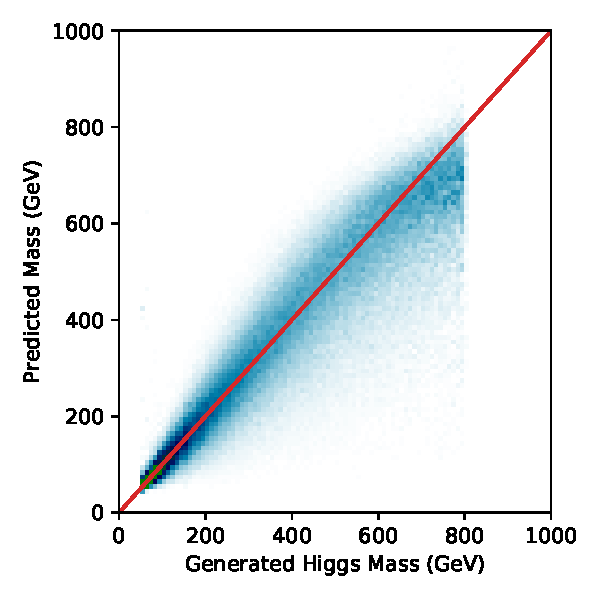
\includegraphics[width=8cm]{\PhDthesisdir/plots_and_images/my_plots/ML/from_ML_plots/trained_NNs_FastSim/DeepTau-inclusive/PuppiMET_with_METcov_j1j2jr_Nnu_Npu/predicted_vs_answers_histo-NN-ADAM_glorot_uniform-activation-softplus-batch_size-2048-mape-Adadelta-u-inclusive-3-layers-1000-neurons-en.pdf}};

\draw [ltcolororange, thick] (6.225, 1.2) -- (6.225, 7.5);
\draw (6.225, 6.3) node [ltcolororange, rotate=90, below left] {area 2};
\draw [ltcolororange, thick] (1.9, 1.2) -- (1.9, 7.5);
\draw (2.0, 1.5) node [ltcolororange, rotate=90, above right] {area 1};

\draw [ltcolorviolet, thick] (6.2,6.3) -- (1.6,3.75);
\draw [ltcolorviolet, thick] (1.9,1.5) -- (6.2,3.75);
\draw (3.5, 4.7) node [ltcolorviolet, rotate=27.5, above] {area 3};
\draw (3.5, 2.4) node [ltcolorviolet, rotate=27.5, below] {area 4};

\draw (4,3.85) node [ltcoloryellow3, rotate=27.5] {area 5};
\end{tikzpicture}
